% Options for packages loaded elsewhere
\PassOptionsToPackage{unicode}{hyperref}
\PassOptionsToPackage{hyphens}{url}
%
\documentclass[
  letterpaper,
]{book}

\usepackage{amsmath,amssymb}
\usepackage{iftex}
\ifPDFTeX
  \usepackage[T1]{fontenc}
  \usepackage[utf8]{inputenc}
  \usepackage{textcomp} % provide euro and other symbols
\else % if luatex or xetex
  \usepackage{unicode-math}
  \defaultfontfeatures{Scale=MatchLowercase}
  \defaultfontfeatures[\rmfamily]{Ligatures=TeX,Scale=1}
\fi
\usepackage{lmodern}
\ifPDFTeX\else  
    % xetex/luatex font selection
\fi
% Use upquote if available, for straight quotes in verbatim environments
\IfFileExists{upquote.sty}{\usepackage{upquote}}{}
\IfFileExists{microtype.sty}{% use microtype if available
  \usepackage[]{microtype}
  \UseMicrotypeSet[protrusion]{basicmath} % disable protrusion for tt fonts
}{}
\makeatletter
\@ifundefined{KOMAClassName}{% if non-KOMA class
  \IfFileExists{parskip.sty}{%
    \usepackage{parskip}
  }{% else
    \setlength{\parindent}{0pt}
    \setlength{\parskip}{6pt plus 2pt minus 1pt}}
}{% if KOMA class
  \KOMAoptions{parskip=half}}
\makeatother
\usepackage{xcolor}
\setlength{\emergencystretch}{3em} % prevent overfull lines
\setcounter{secnumdepth}{5}
% Make \paragraph and \subparagraph free-standing
\ifx\paragraph\undefined\else
  \let\oldparagraph\paragraph
  \renewcommand{\paragraph}[1]{\oldparagraph{#1}\mbox{}}
\fi
\ifx\subparagraph\undefined\else
  \let\oldsubparagraph\subparagraph
  \renewcommand{\subparagraph}[1]{\oldsubparagraph{#1}\mbox{}}
\fi


\providecommand{\tightlist}{%
  \setlength{\itemsep}{0pt}\setlength{\parskip}{0pt}}\usepackage{longtable,booktabs,array}
\usepackage{calc} % for calculating minipage widths
% Correct order of tables after \paragraph or \subparagraph
\usepackage{etoolbox}
\makeatletter
\patchcmd\longtable{\par}{\if@noskipsec\mbox{}\fi\par}{}{}
\makeatother
% Allow footnotes in longtable head/foot
\IfFileExists{footnotehyper.sty}{\usepackage{footnotehyper}}{\usepackage{footnote}}
\makesavenoteenv{longtable}
\usepackage{graphicx}
\makeatletter
\def\maxwidth{\ifdim\Gin@nat@width>\linewidth\linewidth\else\Gin@nat@width\fi}
\def\maxheight{\ifdim\Gin@nat@height>\textheight\textheight\else\Gin@nat@height\fi}
\makeatother
% Scale images if necessary, so that they will not overflow the page
% margins by default, and it is still possible to overwrite the defaults
% using explicit options in \includegraphics[width, height, ...]{}
\setkeys{Gin}{width=\maxwidth,height=\maxheight,keepaspectratio}
% Set default figure placement to htbp
\makeatletter
\def\fps@figure{htbp}
\makeatother

\makeatletter
\makeatother
\makeatletter
\@ifpackageloaded{bookmark}{}{\usepackage{bookmark}}
\makeatother
\makeatletter
\@ifpackageloaded{caption}{}{\usepackage{caption}}
\AtBeginDocument{%
\ifdefined\contentsname
  \renewcommand*\contentsname{Table of contents}
\else
  \newcommand\contentsname{Table of contents}
\fi
\ifdefined\listfigurename
  \renewcommand*\listfigurename{List of Figures}
\else
  \newcommand\listfigurename{List of Figures}
\fi
\ifdefined\listtablename
  \renewcommand*\listtablename{List of Tables}
\else
  \newcommand\listtablename{List of Tables}
\fi
\ifdefined\figurename
  \renewcommand*\figurename{Figure}
\else
  \newcommand\figurename{Figure}
\fi
\ifdefined\tablename
  \renewcommand*\tablename{Table}
\else
  \newcommand\tablename{Table}
\fi
}
\@ifpackageloaded{float}{}{\usepackage{float}}
\floatstyle{ruled}
\@ifundefined{c@chapter}{\newfloat{codelisting}{h}{lop}}{\newfloat{codelisting}{h}{lop}[chapter]}
\floatname{codelisting}{Listing}
\newcommand*\listoflistings{\listof{codelisting}{List of Listings}}
\makeatother
\makeatletter
\@ifpackageloaded{caption}{}{\usepackage{caption}}
\@ifpackageloaded{subcaption}{}{\usepackage{subcaption}}
\makeatother
\makeatletter
\@ifpackageloaded{tcolorbox}{}{\usepackage[skins,breakable]{tcolorbox}}
\makeatother
\makeatletter
\@ifundefined{shadecolor}{\definecolor{shadecolor}{rgb}{.97, .97, .97}}
\makeatother
\makeatletter
\makeatother
\makeatletter
\makeatother
\ifLuaTeX
  \usepackage{selnolig}  % disable illegal ligatures
\fi
\IfFileExists{bookmark.sty}{\usepackage{bookmark}}{\usepackage{hyperref}}
\IfFileExists{xurl.sty}{\usepackage{xurl}}{} % add URL line breaks if available
\urlstyle{same} % disable monospaced font for URLs
\hypersetup{
  pdftitle={Sprengel Publication Prototype},
  pdfauthor={Ina},
  hidelinks,
  pdfcreator={LaTeX via pandoc}}

\title{Sprengel Publication Prototype}
\author{Ina}
\date{2023-04-27}

\begin{document}
\frontmatter
\maketitle
\ifdefined\Shaded\renewenvironment{Shaded}{\begin{tcolorbox}[boxrule=0pt, frame hidden, interior hidden, breakable, enhanced, sharp corners, borderline west={3pt}{0pt}{shadecolor}]}{\end{tcolorbox}}\fi

\renewcommand*\contentsname{Table of contents}
{
\setcounter{tocdepth}{2}
\tableofcontents
}
\mainmatter
\bookmarksetup{startatroot}

\hypertarget{part-of-the-series-baroque-toc}{%
\chapter{Part of the series: Baroque
TOC}\label{part-of-the-series-baroque-toc}}

\href{https://nfdi4culture.github.io/class-ADA-CP-pipeline/}{Programme
instructions}

2023-03-17 v1.0

Example publications:

\begin{itemize}
\item
  Exhibition Catalogue (Work in progress) -
  https://nfdi4culture.github.io/catalogue-003/ (content from the
  current repo)
\item
  \href{https://nfdi4culture.github.io/experimental-books-workshop/}{Exhibition
  catalogue demo: toc Baroque /toc} from Experimental Books --
  Re-imagining Scholarly Publishing, COPIM. Workshop URL:
  https://experimentalbooks.pubpub.org/programme-overview
\item
  \href{https://simonxix.github.io/scholarled_catalogue/}{Publishers
  catalogue demo: ScholarLed} A catalogue of ScholarLed presses built on
  a Quarto / Jupyter Notebook model for computational publishing. The
  publication is automatically updated daily to reflect any new books
  added by the publishers.
\item
  \href{https://nfdi4culture.github.io/cp4c/}{Proof of concept \#1} -
  Computational Publication: Computational Publishing for Collections -
  ADA CP Prototype \#1 - Nov 22
\item
  \href{https://nfdi4culture.github.io/art_catalogue_test/}{Proof of
  concept \#2} - To be confirmed, completion for end of April 2023. This
  contains all parts fully rendered: Cover, colophon, essay, collection,
  graph, TIB AV Portal, Semantic Kompakkt
\item
  semanticClimate: To be confirmed - customised research papers readers
  made for regional climate change action plans based on IPCC reports
  and sourcing content from open research repositories.
\item
  FSCI Summer School - publishing from collections class: To be
  confirmed, July 2023
\end{itemize}

This work is licensed under a Creative Commons Attribution-ShareAlike
4.0 International License.

\bookmarksetup{startatroot}

\hypertarget{colophon}{%
\chapter{Colophon}\label{colophon}}

Fork title:

Author:

ORCID:

Date:

DOI:

Repositor:

PUBLISHING FROM COLLECTIONS USES OF COMPUTATIONAL PUBLISHIGN AND
LINKEDOPEN DATA

Open Science Lab - TIB Hannnover

First published 2023-03-30

Copyright © The Authors 2023 Licensed as
https://creativecommons.org/licenses/by-sa/4.0/

DOI: https://doi.org/10.5281/zenodo.7701161

\bookmarksetup{startatroot}

\hypertarget{sprengel-museum}{%
\chapter{Sprengel Museum}\label{sprengel-museum}}

Source: ChatGPT

The Sprengel Museum Hannover is one of the most significant museums of
modern art in Germany. Located in the heart of the city of Hannover, the
museum houses a diverse collection of modern and contemporary art that
spans the 20th and 21st centuries.

The museum's collection includes works from renowned artists such as
Pablo Picasso, Paul Klee, Max Ernst, and Salvador Dali, among others.
The collection is particularly strong in German Expressionism and the
Bauhaus movement, with many important works by artists such as Max
Beckmann, Otto Dix, and Lyonel Feininger.

In addition to its impressive collection of paintings, the museum also
has a substantial collection of graphic art and photography. The graphic
art collection includes works by Edvard Munch, Wassily Kandinsky, and
Kurt Schwitters.

\hypertarget{opening-up-collections}{%
\section{Opening up collections}\label{opening-up-collections}}

The Sprengel Museum Hannover has made a significant portion of its
collection available to the public through Wikimedia Commons, a free
online repository of images, videos, and other media files. As of my
knowledge cutoff date of 2021, there were over 1,700 images of artworks
from the museum's collection available on Wikimedia Commons.

The museum's decision to share its collection on Wikimedia Commons
reflects a commitment to making art more accessible and available to a
wider audience. By allowing free access to high-quality images of its
collection, the Sprengel Museum Hannover is providing an invaluable
resource for students, researchers, and art lovers around the world.

In summary, the Sprengel Museum Hannover's decision to make a
significant portion of its collection available on Wikimedia Commons is
a testament to its commitment to education and accessibility, and it is
a valuable resource for anyone interested in the study and appreciation
of modern and contemporary art.

\hypertarget{wikidata}{%
\subsection{Wikidata}\label{wikidata}}

In addition to making a significant portion of its collection available
on Wikimedia Commons, the Sprengel Museum Hannover has also contributed
to Wikidata, a free and open knowledge base that provides structured
data and information for a wide range of topics, including art and
cultural heritage.

By contributing to Wikidata, the Sprengel Museum Hannover has made
information about its collection more easily accessible and discoverable
for researchers, scholars, and art enthusiasts. As of my knowledge
cutoff date of 2021, the museum had contributed information on over
4,700 objects to Wikidata, including artworks, photographs, and other
cultural artifacts.

The data available on Wikidata includes information on the artists who
created the works, the materials and techniques used, the provenance and
history of the objects, and other relevant information. This information
can be used to gain a deeper understanding of the objects and their
place in the history of modern and contemporary art.

In addition to providing valuable information to researchers and art
enthusiasts, the museum's contributions to Wikidata also reflect its
commitment to open access and collaboration. By sharing information
about its collection on a freely accessible platform, the Sprengel
Museum Hannover is helping to promote the exchange of knowledge and
ideas in the field of art and cultural heritage.

\bookmarksetup{startatroot}

\hypertarget{my-customized-paintings-catalogue-in-jupyter-notebook}{%
\chapter{My customized Paintings catalogue in Jupyter
Notebook}\label{my-customized-paintings-catalogue-in-jupyter-notebook}}

Objective: Make a selection of nine paintings for the exhibition
catalogue to be selected from Wikidata and rendered multi-format in
Quarto.

The below Python code uses SPARQLWrapper to retrieve data from Wikidata
based on a SPARQL query.

Wikidata link: \url{http://www.wikidata.org/entity/Q934482}

Title: The Street Enters the House

Year: 1911

Creator: Umberto Boccioni

Copyright: public domain

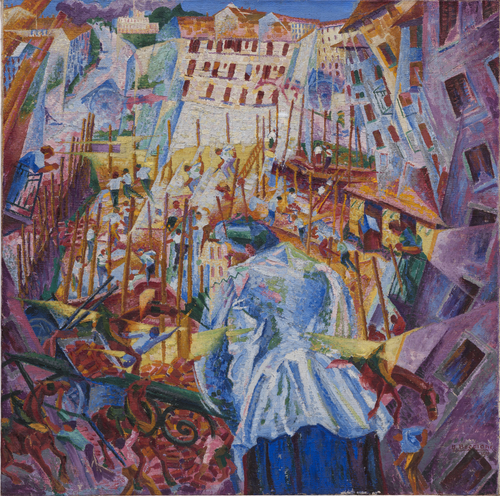
\includegraphics{paintings_1_files/figure-pdf/cell-2-output-2.png}

Wikidata link: \url{http://www.wikidata.org/entity/Q18890767}

Title: Seated Nude

Year: 1902

Creator: Edvard Munch

Copyright: public domain

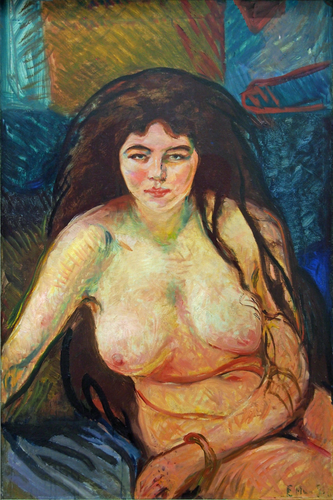
\includegraphics{paintings_1_files/figure-pdf/cell-2-output-4.png}

Wikidata link: \url{http://www.wikidata.org/entity/Q18890869}

Title: Small Town Street in Snow

Year: 1906

Creator: Edvard Munch

Copyright: public domain

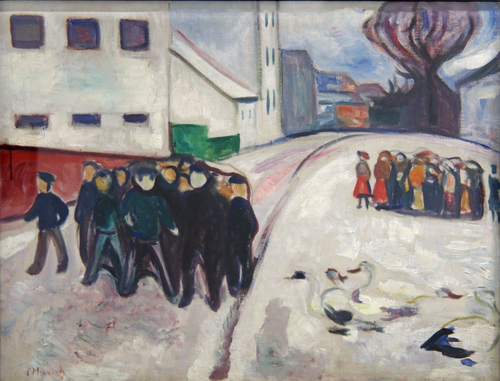
\includegraphics{paintings_1_files/figure-pdf/cell-2-output-6.png}

Wikidata link: \url{http://www.wikidata.org/entity/Q30005098}

Title: Women in Black

Year: 1910

Creator: Marianne von Werefkin

Copyright: public domain

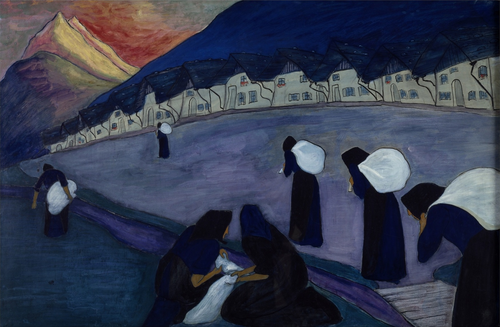
\includegraphics{paintings_1_files/figure-pdf/cell-2-output-8.png}

Wikidata link: \url{http://www.wikidata.org/entity/Q52086842}

Title: Horses and Eagle

Year: 1912

Creator: Franz Marc

Copyright: public domain

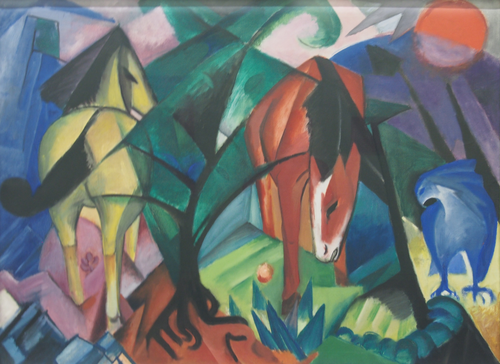
\includegraphics{paintings_1_files/figure-pdf/cell-2-output-10.png}

Wikidata link: \url{http://www.wikidata.org/entity/Q52086847}

Title: Small Composition II

Year: 1914

Creator: Franz Marc

Copyright: public domain

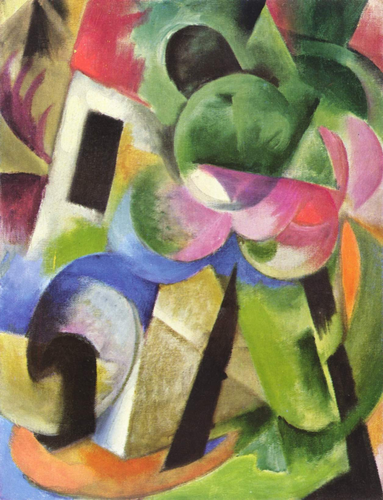
\includegraphics{paintings_1_files/figure-pdf/cell-2-output-12.png}

Wikidata link: \url{http://www.wikidata.org/entity/Q54366255}

Title: Large Bright Showcase

Year: 1912

Creator: August Macke

Copyright: public domain

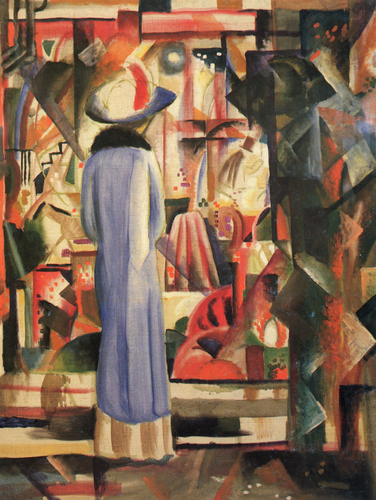
\includegraphics{paintings_1_files/figure-pdf/cell-2-output-14.png}

\bookmarksetup{startatroot}

\hypertarget{activity-paintings-catalogue-in-jupyter-notebook}{%
\chapter{Activity: Paintings catalogue in Jupyter
Notebook}\label{activity-paintings-catalogue-in-jupyter-notebook}}

https://w.wiki/6cAJ

\{`item': \{`type': `uri', `value':
`http://www.wikidata.org/entity/Q934482'\}, `image': \{`type': `uri',
`value':
`http://commons.wikimedia.org/wiki/Special:FilePath/Umberto\%20Boccioni\%2C\%201911\%2C\%20The\%20Street\%20Enters\%20the\%20House\%2C\%20oil\%20on\%20canvas\%2C\%20100\%20x\%20100.6\%20cm\%2C\%20Sprengel\%20Museum.jpg'\},
`creator': \{`type': `uri', `value':
`http://www.wikidata.org/entity/Q152797'\}, `inception': \{`datatype':
`http://www.w3.org/2001/XMLSchema\#dateTime', `type': `literal',
`value': `1911-01-01T00:00:00Z'\}, `itemLabel': \{`xml:lang': `en',
`type': `literal', `value': `The Street Enters the House'\},
`creatorLabel': \{`xml:lang': `en', `type': `literal', `value': `Umberto
Boccioni'\}\} \{`item': \{`type': `uri', `value':
`http://www.wikidata.org/entity/Q1871122'\}, `creator': \{`type': `uri',
`value': `http://www.wikidata.org/entity/Q703331'\}, `inception':
\{`datatype': `http://www.w3.org/2001/XMLSchema\#dateTime', `type':
`literal', `value': `1927-01-01T00:00:00Z'\}, `itemLabel': \{`type':
`literal', `value': `Q1871122'\}, `creatorLabel': \{`xml:lang': `en',
`type': `literal', `value': `Christian Schad'\}\} \{`item': \{`type':
`uri', `value': `http://www.wikidata.org/entity/Q17143943'\}, `creator':
\{`type': `uri', `value': `http://www.wikidata.org/entity/Q152788'\},
`itemLabel': \{`xml:lang': `en', `type': `literal', `value': `Stormy
Sea'\}, `creatorLabel': \{`xml:lang': `en', `type': `literal', `value':
`Emil Nolde'\}\} \{`item': \{`type': `uri', `value':
`http://www.wikidata.org/entity/Q18890767'\}, `image': \{`type': `uri',
`value':
`http://commons.wikimedia.org/wiki/Special:FilePath/Munch\%20Edvard\%20Weiblicher\%20Halbakt\%20Sprengel\%20Museum\%2001.JPG'\},
`creator': \{`type': `uri', `value':
`http://www.wikidata.org/entity/Q41406'\}, `inception': \{`datatype':
`http://www.w3.org/2001/XMLSchema\#dateTime', `type': `literal',
`value': `1902-01-01T00:00:00Z'\}, `itemLabel': \{`xml:lang': `en',
`type': `literal', `value': `Seated Nude'\}, `creatorLabel':
\{`xml:lang': `en', `type': `literal', `value': `Edvard Munch'\}\}
\{`item': \{`type': `uri', `value':
`http://www.wikidata.org/entity/Q18890869'\}, `image': \{`type': `uri',
`value':
`http://commons.wikimedia.org/wiki/Special:FilePath/Munch\%20Edward\%20Elgersburg\%20Sprengel\%20Museum\%2001.JPG'\},
`creator': \{`type': `uri', `value':
`http://www.wikidata.org/entity/Q41406'\}, `inception': \{`datatype':
`http://www.w3.org/2001/XMLSchema\#dateTime', `type': `literal',
`value': `1906-01-01T00:00:00Z'\}, `itemLabel': \{`xml:lang': `en',
`type': `literal', `value': `Small Town Street in Snow'\},
`creatorLabel': \{`xml:lang': `en', `type': `literal', `value': `Edvard
Munch'\}\} \{`item': \{`type': `uri', `value':
`http://www.wikidata.org/entity/Q20087550'\}, `creator': \{`type':
`uri', `value': `http://www.wikidata.org/entity/Q168704'\}, `inception':
\{`datatype': `http://www.w3.org/2001/XMLSchema\#dateTime', `type':
`literal', `value': `1972-01-01T00:00:00Z'\}, `itemLabel': \{`xml:lang':
`en', `type': `literal', `value': `Death of the Patriarch'\},
`creatorLabel': \{`xml:lang': `en', `type': `literal', `value': `Niki de
Saint Phalle'\}\} \{`item': \{`type': `uri', `value':
`http://www.wikidata.org/entity/Q20087564'\}, `creator': \{`type':
`uri', `value': `http://www.wikidata.org/entity/Q168704'\}, `inception':
\{`datatype': `http://www.w3.org/2001/XMLSchema\#dateTime', `type':
`literal', `value': `1954-01-01T00:00:00Z'\}, `itemLabel': \{`xml:lang':
`en', `type': `literal', `value': `Family portrait'\}, `creatorLabel':
\{`xml:lang': `en', `type': `literal', `value': `Niki de Saint
Phalle'\}\} \{`item': \{`type': `uri', `value':
`http://www.wikidata.org/entity/Q27061960'\}, `image': \{`type': `uri',
`value':
`http://commons.wikimedia.org/wiki/Special:FilePath/M\%C3\%BCller\%20Otto\%20Drei\%20Akte\%20im\%20Wald\%20Sprengel\%20Museum\%2001.JPG'\},
`creator': \{`type': `uri', `value':
`http://www.wikidata.org/entity/Q1307060'\}, `inception': \{`datatype':
`http://www.w3.org/2001/XMLSchema\#dateTime', `type': `literal',
`value': `1911-01-01T00:00:00Z'\}, `itemLabel': \{`xml:lang': `en',
`type': `literal', `value': `Three Nudes in the Forest'\},
`creatorLabel': \{`xml:lang': `en', `type': `literal', `value': `Otto
Müller'\}\} \{`item': \{`type': `uri', `value':
`http://www.wikidata.org/entity/Q27533742'\}, `creator': \{`type':
`uri', `value': `http://www.wikidata.org/entity/Q161143'\}, `inception':
\{`datatype': `http://www.w3.org/2001/XMLSchema\#dateTime', `type':
`literal', `value': `1922-01-01T00:00:00Z'\}, `itemLabel': \{`xml:lang':
`en', `type': `literal', `value': `Windmill'\}, `creatorLabel':
\{`xml:lang': `en', `type': `literal', `value': `Karl
Schmidt-Rottluff'\}\} \{`item': \{`type': `uri', `value':
`http://www.wikidata.org/entity/Q30005098'\}, `image': \{`type': `uri',
`value':
`http://commons.wikimedia.org/wiki/Special:FilePath/Marianne\%20von\%20Werefkin\%20-\%20Schwarze\%20Frauen\%20\%281910\%29.jpg'\},
`creator': \{`type': `uri', `value':
`http://www.wikidata.org/entity/Q464016'\}, `inception': \{`datatype':
`http://www.w3.org/2001/XMLSchema\#dateTime', `type': `literal',
`value': `1910-01-01T00:00:00Z'\}, `itemLabel': \{`xml:lang': `en',
`type': `literal', `value': `Women in Black'\}, `creatorLabel':
\{`xml:lang': `en', `type': `literal', `value': `Marianne von
Werefkin'\}\} \{`item': \{`type': `uri', `value':
`http://www.wikidata.org/entity/Q52086842'\}, `image': \{`type': `uri',
`value':
`http://commons.wikimedia.org/wiki/Special:FilePath/Marc\%20Franz\%20Pferde\%20und\%20Adler\%20Sprengel\%20Museum\%2001.JPG'\},
`creator': \{`type': `uri', `value':
`http://www.wikidata.org/entity/Q44054'\}, `inception': \{`datatype':
`http://www.w3.org/2001/XMLSchema\#dateTime', `type': `literal',
`value': `1912-01-01T00:00:00Z'\}, `itemLabel': \{`xml:lang': `en',
`type': `literal', `value': `Horses and Eagle'\}, `creatorLabel':
\{`xml:lang': `en', `type': `literal', `value': `Franz Marc'\}\}
\{`item': \{`type': `uri', `value':
`http://www.wikidata.org/entity/Q52086847'\}, `image': \{`type': `uri',
`value':
`http://commons.wikimedia.org/wiki/Special:FilePath/Franz\%20Marc\%20014.jpg'\},
`creator': \{`type': `uri', `value':
`http://www.wikidata.org/entity/Q44054'\}, `inception': \{`datatype':
`http://www.w3.org/2001/XMLSchema\#dateTime', `type': `literal',
`value': `1914-01-01T00:00:00Z'\}, `itemLabel': \{`xml:lang': `en',
`type': `literal', `value': `Small Composition II'\}, `creatorLabel':
\{`xml:lang': `en', `type': `literal', `value': `Franz Marc'\}\}
\{`item': \{`type': `uri', `value':
`http://www.wikidata.org/entity/Q54366255'\}, `image': \{`type': `uri',
`value':
`http://commons.wikimedia.org/wiki/Special:FilePath/August\%20Macke\%20016.jpg'\},
`creator': \{`type': `uri', `value':
`http://www.wikidata.org/entity/Q33981'\}, `inception': \{`datatype':
`http://www.w3.org/2001/XMLSchema\#dateTime', `type': `literal',
`value': `1912-01-01T00:00:00Z'\}, `itemLabel': \{`xml:lang': `en',
`type': `literal', `value': `Large Bright Showcase'\}, `creatorLabel':
\{`xml:lang': `en', `type': `literal', `value': `August Macke'\}\}
\{`item': \{`type': `uri', `value':
`http://www.wikidata.org/entity/Q65159258'\}, `image': \{`type': `uri',
`value':
`http://commons.wikimedia.org/wiki/Special:FilePath/Otto\%20Mueller\%20-\%20Liebespaar\%20-\%20ca1920.jpeg'\},
`creator': \{`type': `uri', `value':
`http://www.wikidata.org/entity/Q317041'\}, `inception': \{`datatype':
`http://www.w3.org/2001/XMLSchema\#dateTime', `type': `literal',
`value': `1920-01-01T00:00:00Z'\}, `itemLabel': \{`xml:lang': `en',
`type': `literal', `value': `Lovers'\}, `creatorLabel': \{`xml:lang':
`en', `type': `literal', `value': `Otto Mueller'\}\} \{`item': \{`type':
`uri', `value': `http://www.wikidata.org/entity/Q105592817'\}, `image':
\{`type': `uri', `value':
`http://commons.wikimedia.org/wiki/Special:FilePath/Clown-Acrobat\%20.jpg'\},
`creator': \{`type': `uri', `value':
`http://www.wikidata.org/entity/Q164683'\}, `inception': \{`datatype':
`http://www.w3.org/2001/XMLSchema\#dateTime', `type': `literal',
`value': `1944-01-01T00:00:00Z'\}, `itemLabel': \{`xml:lang': `en',
`type': `literal', `value': `Half Nude Clown'\}, `creatorLabel':
\{`xml:lang': `en', `type': `literal', `value': `Max Beckmann'\}\}
\{`item': \{`type': `uri', `value':
`http://www.wikidata.org/entity/Q111366491'\}, `image': \{`type': `uri',
`value':
`http://commons.wikimedia.org/wiki/Special:FilePath/Beckmann\%20-\%20Self-portrait\%20-\%201899\%20-\%20Sprengel\%20Museum\%20Hannover.jpg'\},
`creator': \{`type': `uri', `value':
`http://www.wikidata.org/entity/Q164683'\}, `inception': \{`datatype':
`http://www.w3.org/2001/XMLSchema\#dateTime', `type': `literal',
`value': `1899-01-01T00:00:00Z'\}, `itemLabel': \{`type': `literal',
`value': `Q111366491'\}, `creatorLabel': \{`xml:lang': `en', `type':
`literal', `value': `Max Beckmann'\}\} \{`item': \{`type': `uri',
`value': `http://www.wikidata.org/entity/Q113492912'\}, `creator':
\{`type': `uri', `value': `http://www.wikidata.org/entity/Q164712'\},
`inception': \{`datatype': `http://www.w3.org/2001/XMLSchema\#dateTime',
`type': `literal', `value': `1936-01-01T00:00:00Z'\}, `itemLabel':
\{`xml:lang': `en', `type': `literal', `value': `Procession in Lace'\},
`creatorLabel': \{`xml:lang': `en', `type': `literal', `value': `Paul
Delvaux'\}\}


\backmatter

\end{document}
